%#!uplatex
%%%%%%%%%%%%%%%%%%%%%%%%%%%%%%%%%%%%%%%%%%%%%%%%%%%%%%%%%%%%%%%%%%%%%%%%%%%%%%%%%%%%%%%%%%%%%%%%%%%
%%%%%%%%%%%%%%%%%%%%%%%%%%%%%%%%%%%%%%%%%%%%%%%%%%%%%%%%%%%%%%%%%%%%%%%%%%%%%%%%%%%%%%%%%%%%%%%%%%%
%%%%%%%%%%%%%%%%%%%%%%%%%%%%%%%%%%%%%%%%%%%%%%%%%%%%%%%%%%%%%%%%%%%%%%%%%%%%%%%%%%%%%%%%%%%%%%%%%%%
\documentclass[12pt,dvipdfmx,uplatex]{beamer}
%%%%%%%%%%%%%%%%%%%%%%%%%%%%%%%%%%%%%%%%%%%%%%%%%%%%%%%%%%%%%%%%%%%%%%%%%%%%%%%%%%%%%%%%%%%%%%%%%%%
%%%%%%%%%%%%%%%%%%%%%%%%%%%%%%%%%%%%%%%%%%%%%%%%%%%%%%%%%%%%%%%%%%%%%%%%%%%%%%%%%%%%%%%%%%%%%%%%%%%
%%%%%%%%%%%%%%%%%%%%%%%%%%%%%%%%%%%%%%%%%%%%%%%%%%%%%%%%%%%%%%%%%%%%%%%%%%%%%%%%%%%%%%%%%%%%%%%%%%%
%%%
%%% hyperref 文字化け対策
%%%
\usepackage{pxjahyper}
\usepackage{hyperref}
%%%%%%%%%%%%%%%%%%%%%%%%%%%%%%%%%%%%%%%%%%%%%%%%%%%%%%%%%%%%%%%%%%%%%%%%%%%%%%%%%%%%%%%%%%%%%%%%%%%
%%%%%%%%%%%%%%%%%%%%%%%%%%%%%%%%%%%%%%%%%%%%%%%%%%%%%%%%%%%%%%%%%%%%%%%%%%%%%%%%%%%%%%%%%%%%%%%%%%%
%%%%%%%%%%%%%%%%%%%%%%%%%%%%%%%%%%%%%%%%%%%%%%%%%%%%%%%%%%%%%%%%%%%%%%%%%%%%%%%%%%%%%%%%%%%%%%%%%%%
%%%
%%% 各種パッケージ
%%%
\usepackage{graphicx}
%\usepackage{url,cite}
\usepackage{amsmath}
\usepackage{amsthm} \theoremstyle{definition} %theorem環境が斜体になるので注意
\usepackage{amssymb} % AMS-TeX
\usepackage{setspace}
\usepackage{multirow}
\usepackage{udline} % udline.sty

%%%%%%%%%%%%%%%%%%%%%%%%%%%%%%%%%%%%%%%%%%%%%%%%%%%%%%%%%%%%%%%%%%%%%%%%%%%%%%%%%%%%%%%%%%%%%%%%%%%
%%%%%%%%%%%%%%%%%%%%%%%%%%%%%%%%%%%%%%%%%%%%%%%%%%%%%%%%%%%%%%%%%%%%%%%%%%%%%%%%%%%%%%%%%%%%%%%%%%%
%%%%%%%%%%%%%%%%%%%%%%%%%%%%%%%%%%%%%%%%%%%%%%%%%%%%%%%%%%%%%%%%%%%%%%%%%%%%%%%%%%%%%%%%%%%%%%%%%%%
%%%
%%% 本文・数式フォント
%%%
\usepackage{newtxtext}
\usepackage[varg]{newtxmath}
%\usepackage{newpxtext}
%\usepackage[varg]{newpxmath}

% \mathcal(\cal)の扱い
%\DeclareMathAlphabet{\mathcal}{OMS}{cmsy}{m}{n} %computer modern
%\DeclareMathAlphabet{\mathcal}{OMS}{txsy}{m}{n} %txfont
%\usepackage[psamsfonts]{eucal} % euler

% mathptmx時に数式モードのvをtxfontから借りる
% \DeclareSymbolFont{lettersA}{U}{txmia}{m}{it}
% \SetSymbolFont{lettersA}{bold}{U}{txmia}{bx}{it}
% \DeclareFontSubstitution{U}{txmia}{m}{it}
% \DeclareMathSymbol{v}{\mathalpha}{lettersA}{"33} %"

%%%%%%%%%%%%%%%%%%%%%%%%%%%%%%%%%%%%%%%%%%%%%%%%%%%%%%%%%%%%%%%%%%%%%%%%%%%%%%%%%%%%%%%%%%%%%%%%%%%
%%%%%%%%%%%%%%%%%%%%%%%%%%%%%%%%%%%%%%%%%%%%%%%%%%%%%%%%%%%%%%%%%%%%%%%%%%%%%%%%%%%%%%%%%%%%%%%%%%%
%%%%%%%%%%%%%%%%%%%%%%%%%%%%%%%%%%%%%%%%%%%%%%%%%%%%%%%%%%%%%%%%%%%%%%%%%%%%%%%%%%%%%%%%%%%%%%%%%%%
%%%
%%%  日本語フォントをゴシックに、数式フォントを太字に変更する
%%%
\usepackage[deluxe]{otf}
\renewcommand{\kanjifamilydefault}{\gtdefault}
\renewcommand{\familydefault}{\sfdefault}

\setbeamerfont{title}{size=\large,series=\bfseries}
\setbeamerfont{frametitle}{size=\large,series=\bfseries}
%\setbeamertemplate{frametitle}[default][center]
\usefonttheme{professionalfonts} 

%%%
% Suppress Warning in the case of uplatex
\DeclareFontShape{JY2}{hgt}{b}{n}{<->ssub*hgt/bx/n}{}
\DeclareFontShape{JT2}{hgt}{b}{n}{<->ssub*hgt/bx/n}{}

%\mathversion{bold} %数式フォントを太字に

%%%%%%%%%%%%%%%%%%%%%%%%%%%%%%%%%%%%%%%%%%%%%%%%%%%%%%%%%%%%%%%%%%%%%%%%%%%%%%%%%%%%%%%%%%%%%%%%%%%%%%
%%% Beamer template preamble
%%%
%%% �ơ��ޤλ��ꡢ��ά���� default �ˤʤ�
%%%

 % �ե졼��λ��ꡢ��ά��
%%%%%%%%%%%%%%%%%%%%%%%%%%%% THEME
  %\usetheme{AnnArbor}
  %\usetheme{Antibes}
  %\usetheme{Bergen}
  %\usetheme{Berkeley}
  %\usetheme{Berlin}
  \usetheme{Boadilla}
  %\usetheme{boxes}
  %\usetheme{CambridgeUS}
  %\usetheme{Copenhagen}
  %\usetheme{Darmstadt}
  %\usetheme{default}
  %\usetheme{Dresden}
  %\usetheme{Frankfurt}
  %\usetheme{Goettingen}
  %\usetheme{Hannover}
  %\usetheme{Ilmenau}
  %\usetheme{JuanLesPins}
  %\usetheme{Luebeck}
  %\usetheme{Madrid}
  %\usetheme{Malmoe}
  %\usetheme{Marburg}
  %\usetheme{Montpellier}
  %\usetheme{PaloAlto}
  %\usetheme{Pittsburgh}
  %\usetheme{Rochester}
  %\usetheme{Singapore}
  %\usetheme{Szeged}
  %\usetheme{Warsaw}

% ����
%%%%%%%%%%%%%%%%%%%%%%%%%%%% COLOR THEME
  %\usecolortheme{albatross}
  %\usecolortheme{beetle}
  %\usecolortheme{crane}
  %\usecolortheme{default}
  %\usecolortheme{dolphin}
  %\usecolortheme{dove}
  %\usecolortheme{fly}
  %\usecolortheme{lily}
  %\usecolortheme{orchid}
  %\usecolortheme{rose}
  %\usecolortheme{seagull}
  %\usecolortheme{seahorse}
  %\usecolortheme{sidebartab}
  %\usecolortheme{structure}
  %\usecolortheme{whale}

% �إå����եå����ե졼��������ꡢ��ά��
  %%%%%%%%%%%%%%%%%%%%%%%%%%%% OUTER THEME
  %\useoutertheme{default}
  %\useoutertheme{infolines}
  %\useoutertheme{miniframes}
  %\useoutertheme{shadow}
  %\useoutertheme{sidebar}
  %\useoutertheme{smoothbars}
  %\useoutertheme{smoothtree}
  %\useoutertheme{split}
  %\useoutertheme{tree}

% �����ȥ롢section, itemize/enumerate �Ķ���
% theorem �Ķ�����, ����ʸ���ʤɤΥ����������ꡢ
% ����
  %%%%%%%%%%%%%%%%%%%%%%%%%%%% INNER THEME
  %\useinnertheme{circles}
  %\useinnertheme{default}
  %\useinnertheme{inmargin}
  \useinnertheme{rectangles}
  %\useinnertheme{rounded}


%\usefonttheme{}	% ����
%\logo{}		% ����
%\logo{\includegraphics[width=2cm]{titech_logo.eps}}

% navi. symbols����Ω���ʤ�����dvipdfmx��Ȥ��ȵ�ǽ���ʤ��Τ���ɽ����
\setbeamertemplate{navigation symbols}{}
%\setbeamertemplate{caption}[numbered]
%%%%%%%%%%%%%%%%%%%%%%%%%%%%%%%%%%%%%%%%%%%%%%%%%%%%%%%%%%%%%%%%%%%%%%%%%%%%%%%%%%%%%%%%%%%%%%%%%%%
%%%%%%%%%%%%%%%%%%%%%%%%%%%%%%%%%%%%%%%%%%%%%%%%%%%%%%%%%%%%%%%%%%%%%%%%%%%%%%%%%%%%%%%%%%%%%%%%%%%
%%%%%%%%%%%%%%%%%%%%%%%%%%%%%%%%%%%%%%%%%%%%%%%%%%%%%%%%%%%%%%%%%%%%%%%%%%%%%%%%%%%%%%%%%%%%%%%%%%%

% \AtBeginSection[] % Do nothing for \section*
% { \begin{frame}<beamer> \frametitle{}
%    \tableofcontents[currentsection,subsectionstyle=hide]
%  \end{frame} } 

%appendix��ڡ���������Ȥ��ʤ�
\newcommand{\backupbegin}{
   \newcounter{framenumberappendix}
   \setcounter{framenumberappendix}{\value{framenumber}}
}
\newcommand{\backupend}{
   \addtocounter{framenumberappendix}{-\value{framenumber}}
   \addtocounter{framenumber}{\value{framenumberappendix}} 
}
% �����Ķ�
% \newtheorem{theorem}{Theorem}
% \newtheorem{lemma}[theorem]{Lemma}
% \newtheorem{corollary}[theorem]{Corollary}
% \newtheorem{definition}[theorem]{Definition}
% \newtheorem{example}[theorem]{Example}
\newtheorem{proposition}{Proposition}
\newtheorem{remark}{Remark}


%%%%%%%%%%%%%%%%%%%%%%%%%%%%%%%%%%%%%%%%%%%%%%%%%%%%%%%%%%%%%%%%%%%%%%%%%%%%%%%%%%%%%%%%%%%%%%%%%%%%%%
% �Ƽ拾�ޥ�������
\def\Fig#1{Fig.\@\ref{#1}}
\def\Table#1{Table~\ref{#1}}
\def\Eq#1{Eq.\@(\ref{#1})}
\def\Eqs#1{Eqs.\@(\ref{#1})}
\def\Thm#1{Theorem~\ref{#1}}
\def\Lma#1{Lemma~\ref{#1}}
\def\Sect#1{Section~\ref{#1}}
\def\Rmk#1{Remark~\ref{#1}}
\def\Prop#1{Proposition~\ref{#1}}
\def\Coro#1{Corollary~\ref{#1}}
\def\Def#1{Definition~\@\ref{#1}}
\def\Prob#1{Problem~\@\ref{#1}}
\def\ie{{i.\@e.\@,~}}
\def\eg{{e.\@g.\@,~}}
\def\etal{{et al.}}

% �����Ķ���
\def\rank{\mathsf{rank}\, }
\def\dim{\mathsf{dim}\, }
\def\rspace{\mathsf{span}}
\def\supp{\mathsf{supp}}
%\def\vec#1{\mathbf{#1}}
\def\F{\mathbb{F}}
\def\wt{\mathsf{wt}}
\def\c{\mathcal{C}}
\def\dc{\mathcal{C}^{\perp}}
\def\d{\mathcal{D}}
\def\dd{\mathcal{D}^{\perp}}
\def\g{\mathcal{G}}
\def\dg{\mathcal{G}^{\perp}}
\def\p{\mathcal{P}}
% \def\rspace{\mathsf{span}}
\def\supp{\mathsf{supp}}
\def\ker{\mathsf{Ker\ }}

%\def\bari#1{\{\widebar{#1}\}}
\def\bari#1{\,\overline{{\!\{#1\}\!}}\,}
%\def\bari#1{\bar{\{#1\}}}
\def\vecxi{Z_{\bari{i}}}
%\def\vecsxi{\vec{z}_i}
\def\tvector{X}
\def\tpackets{X_1,\dots,X_n}
\def\mvector{S}
\def\mpackets{S_1,\dots,S_l}
\def\rvector{Y}
\def\wvector{W}
\def\cvector{C}
\def\cword{C_{1},\dots,C_{l+n}}
\def\pcword{C_{l+1},\dots,C_{l+n}}
\def\randvector{R}

\def\compmat{\Phi}

%\def\vec#1{\mbox{\boldmath $#1$}}

%%%%%%%%%%%%%%%%%%%%%%%%%%%%%%%%%%%%%%%%%%%%%%%%%%%%%%%%%%%%%%%%%%%%%%%%%%%%%%%%%%%%%%%%%%%%%%%%%%%%%%
%���� widebar, Widebar
\usepackage{accents}
\makeatletter
\def\widebar{\accentset{{\cc@style\underline{\mskip11mu}}}}
\makeatother


%%%
%%% 著者など
%%%
\title[Modern Authentication]{Modern Authentication}
\subtitle{FIDO2 Web Authentication (WebAuthn) を学ぶ}
\author[Jun Kurihara]{栗原 淳}
\institute[U-Hyogo/Zettant]{兵庫県立大学 大学院応用情報科学研究科 \\ 株式会社ゼタント}
\date[\today]{\today}

%%%%%%%%%%%%%%%%%%%%%%%%%%%%%%%%%%%%%%%%%%%%%%%%%%%%%%%%%%%%%%%%%%%%%%%%%%%%%%%%%%%%%%%%%%%%%%%%%%%
%%%%%%%%%%%%%%%%%%%%%%%%%%%%%%%%%%%%%%%%%%%%%%%%%%%%%%%%%%%%%%%%%%%%%%%%%%%%%%%%%%%%%%%%%%%%%%%%%%%
%%%%%%%%%%%%%%%%%%%%%%%%%%%%%%%%%%%%%%%%%%%%%%%%%%%%%%%%%%%%%%%%%%%%%%%%%%%%%%%%%%%%%%%%%%%%%%%%%%%
%%%%%%%%%%%%%%%%%%%%%%%%%%%%%%%%%%%%%%%%%%%%%%%%%%%%%%%%%%%%%%%%%%%%%%%%%%%%%%%%%%%%%%%%%%%%%%%%%%%
%%%%%%%%%%%%%%%%%%%%%%%%%%%%%%%%%%%%%%%%%%%%%%%%%%%%%%%%%%%%%%%%%%%%%%%%%%%%%%%%%%%%%%%%%%%%%%%%%%%

\begin{document}

\begin{frame}
\titlepage
\end{frame}

%%%%%%%%%%%%%%%%%%%%%%%%%%%%%%%%%%%%%%%%%%%%%%%%%%%%%%%%%%%%%%%%%%%%%%%%%%%%%%%%%%%%%%%%%%%%%%%%%%%
\section{はじめに}
\begin{frame}
 \centering
 {\Large はじめに}
\end{frame}

\begin{frame}{認証とは}
\begin{block}{認証}
 「何らかの手段」で\alert{対象の正当性を確認する}こと。
\end{block}
\begin{itemize}
 \item メッセージの正当性を確認 $\Rightarrow$ メッセージ認証
 \item サービス利用ユーザの正当性を確認 $\Rightarrow$ ユーザ認証
 \item etc.
\end{itemize}

\vspace{2ex}

※このスライドで単純に「認証」と呼んだときは、\ul{認証対象を「正規ユーザ本人」としたユーザ認証・本人認証を指す}こととする。
\end{frame}

\begin{frame}{本人認証の3つの要素}
本人認証において、正当性確認のため検証されるものは大きく3要素に分類。
\begin{itemize}
 \item \textbf{知識}\\
$\Rightarrow$ 本人しか知らない知識を持っていればOK (ex. パスワード)
 \item \textbf{所有物}\\
$\Rightarrow$ 本人しか持っていない物を提示できればOK (ex. HWキー)
 \item \textbf{生体}\\
$\Rightarrow$ 本人の体の一部を提示できればOK (ex. 指紋)
\end{itemize}
\begin{center}
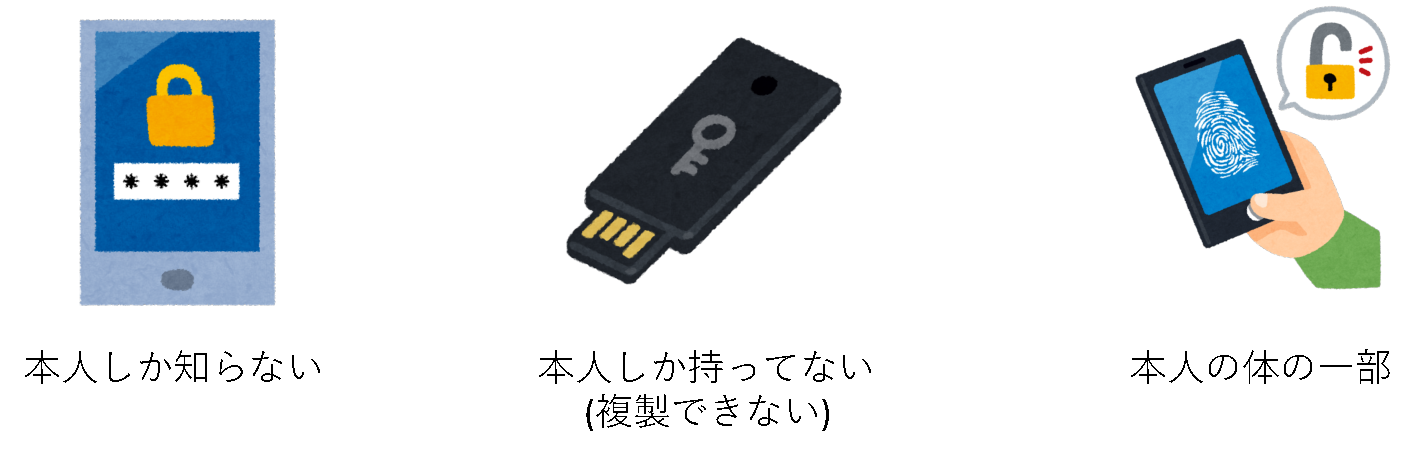
\includegraphics[width=0.7\linewidth]{Figs/auth-three-elements.pdf}
\end{center}

\end{frame}

\begin{frame}{オンラインサービスでのパスワード認証}
\begin{itemize}
\item サービスの利用者の識別子 (ID) と対応するパスワードをサービス事業者に登録、サービス利用時に利用者が自分のIDとパスワードを入力する。
\item パスワードは個人の記憶にのみ存在するため、\alert{パスワードを知っている人はそのサービスに登録してる本人と同一人物}と考えることができる。
\end{itemize}

\begin{center}
おそらく、誰にとっても最も馴染み深い認証方式! 
\end{center}

\end{frame}

\begin{frame}
\begin{figure}
\centering
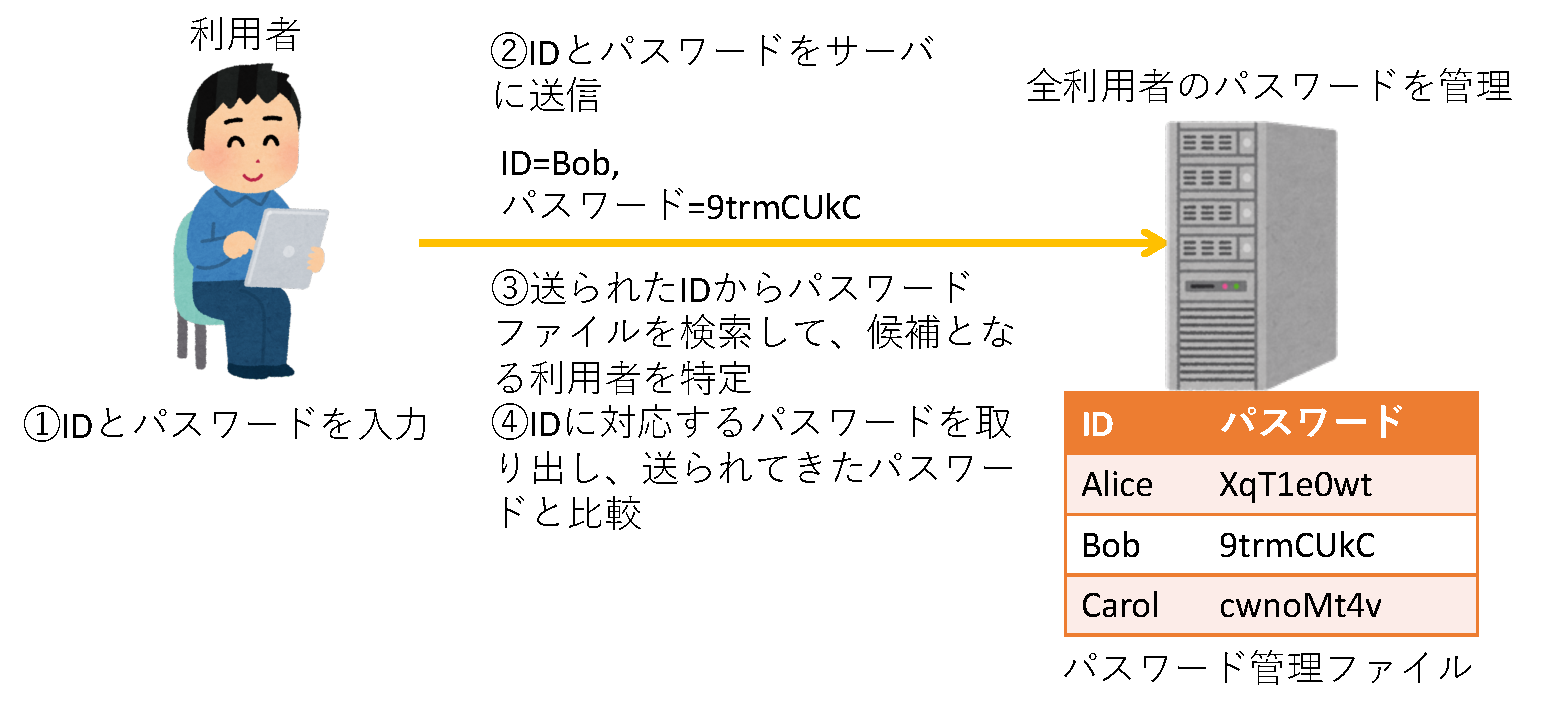
\includegraphics[width=\linewidth]{Figs/password-auth.pdf}\\
\caption{オンラインでの単純なパスワード認証}
\end{figure}
\end{frame}


\begin{frame}{オンラインでのパスワード認証の問題}
英数字・記号を組み合わせたパスワード:
\begin{itemize}
 \item 攻撃者にとって比較的\textbf{予測しやすい}\footnote[frame]{\scriptsize しかもオンラインだと予測→認証トライを繰り返せる}
 \item 「強い」パスワードを使わせるには\textbf{ユーザ教育が必要}\footnote[frame]{\scriptsize 教育なしだと覚え易く「弱い」ものを利用しがち}
 \item \textbf{覚えられない}
 \item etc...
\end{itemize}

\vspace{-5ex}
\begin{center}
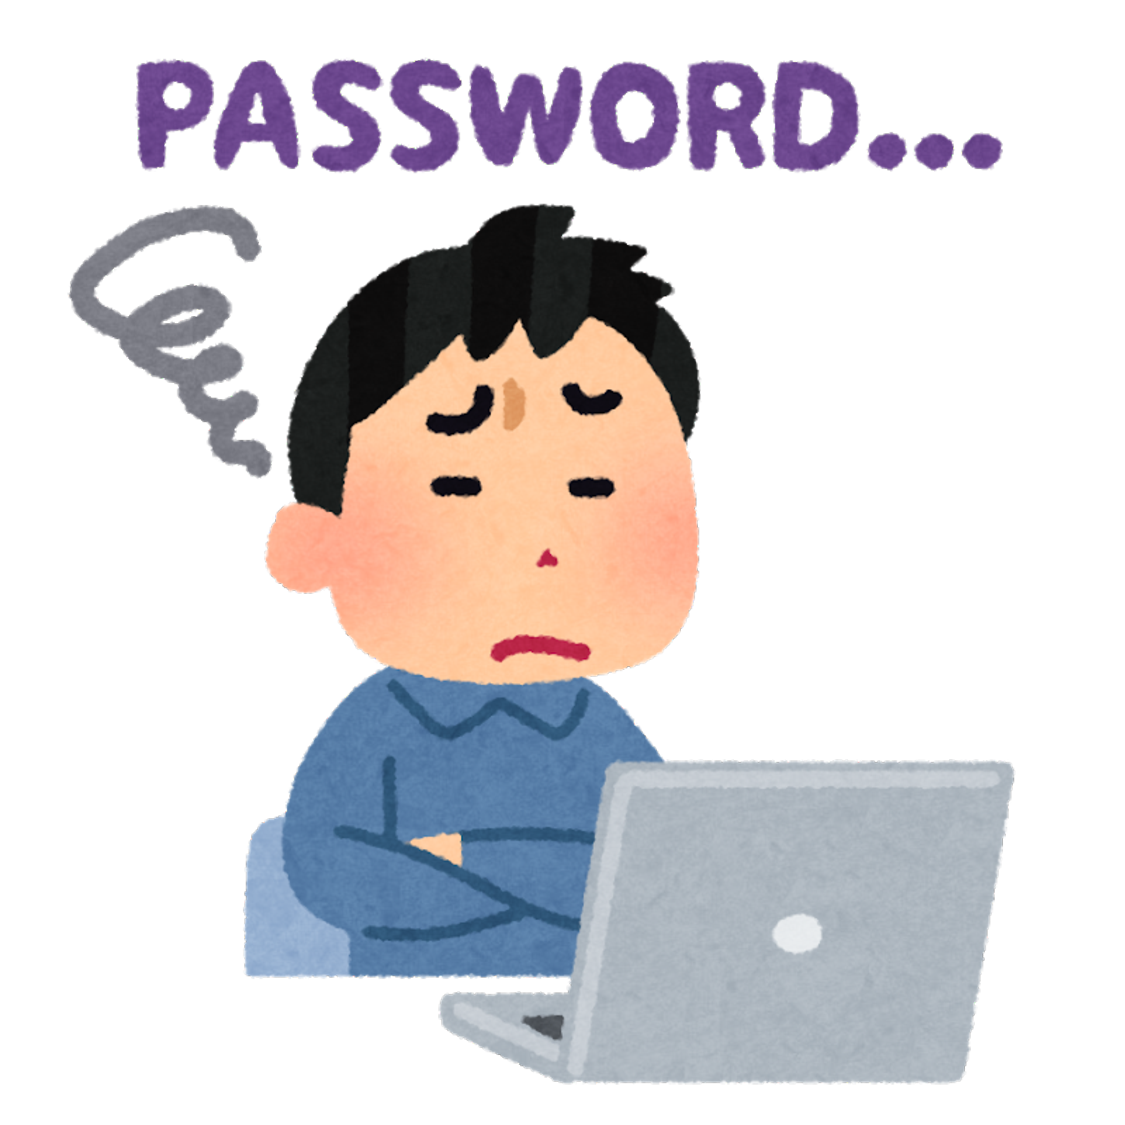
\includegraphics[width=0.2\linewidth]{Figs/password-forget.pdf}
\end{center}
\vspace{-2ex}

\structure{予測できず、誰が使っても強力で、確実に認証できる方法}が必要\\
$\Rightarrow$ \alert{ハードウェアセキュリティキーを使った認証}が人気に\\
$\Rightarrow$ \textbf{FIDOはそのような手法の\ul{標準化された方式}}

\end{frame}

\begin{frame}{FIDO}

\begin{block}{\small FIDO (Fast IDentity Online)}
業界団体FIDO Alliance\footnote[frame]{\scriptsize \url{https://fidoalliance.org}}の策定する、\alert{ハードウェアセキュリティキー+生体認証\footnote[frame]{\scriptsize すなわち、「所有物」と「生体」の二要素を同時に使った認証が可能。}をベースとしたオンラインでの本人認証技術}。
\end{block}

現在はFIDO2 (v2.0) が最新の規格。以降、FIDO2の内容について触れていく。

\vspace{2ex}

厳密には、\structure{FIDO2はパスワードレス認証をサポートしつつも、パスワード+デバイス・生体認証の多要素での認証もサポートする}。

\end{frame}

\begin{frame}{FIDO認証概略}
FIDO認証の特徴:
\begin{itemize}
 \item 公開鍵暗号を利用した、オンラインでの認証方式の提供
 \item 認証器によるローカルでの本人認証
 \item 認証器内部に閉じた署名生成\\ $\Rightarrow$\alert{秘密鍵・パスワード等の秘密情報は外部に出ない}
\end{itemize}
\begin{figure}
\begin{center}
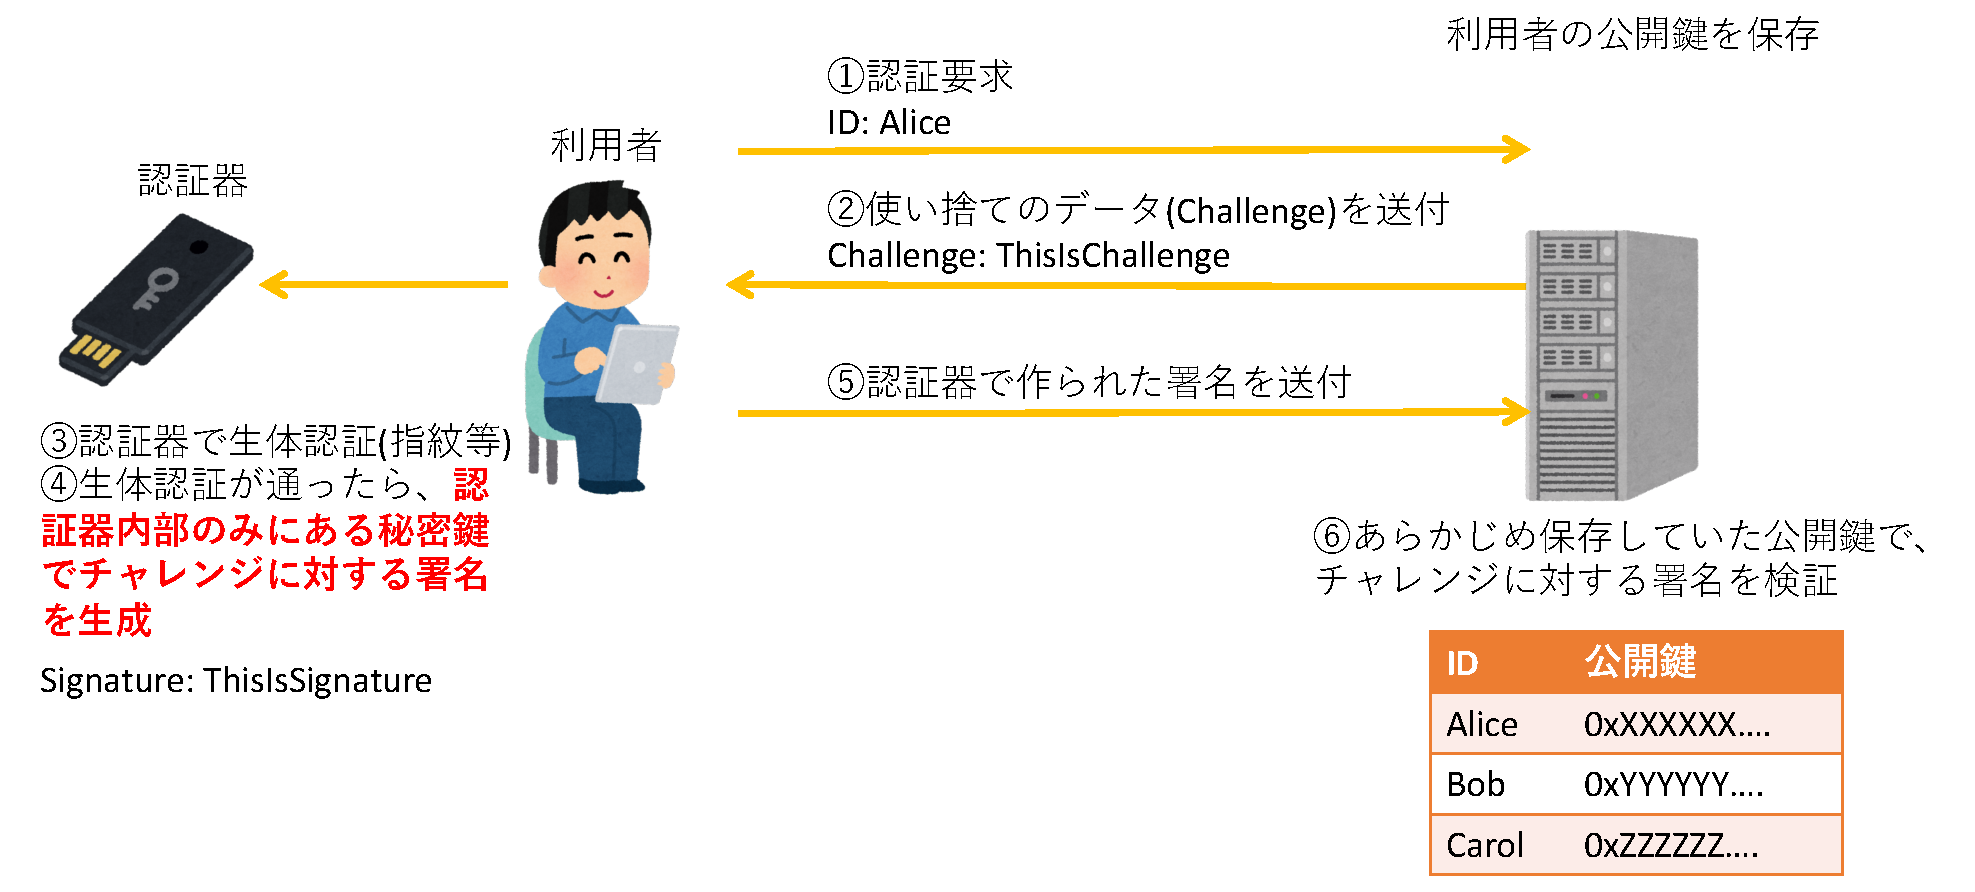
\includegraphics[width=0.9\linewidth]{Figs/FIDO2-auth.pdf}
\caption{FIDO認証概略}
\end{center}
\end{figure}
\end{frame}

\begin{frame}{FIDO2の要素}
FIDO2は、\alert{WebAuthn (Web Authentication)\footnote[frame]{\tiny Spec: \url{https://www.w3.org/TR/webauthn-1/}}と、CTAP (Client-to-Authenticator Protocol)\footnote[frame]{\tiny Spec: \url{https://fidoalliance.org/specs/fido2/fido-client-to-authenticator-protocol-v2.1-rd-20191217.html}}の2つの要素で構成}される。

\begin{figure}
\begin{center}
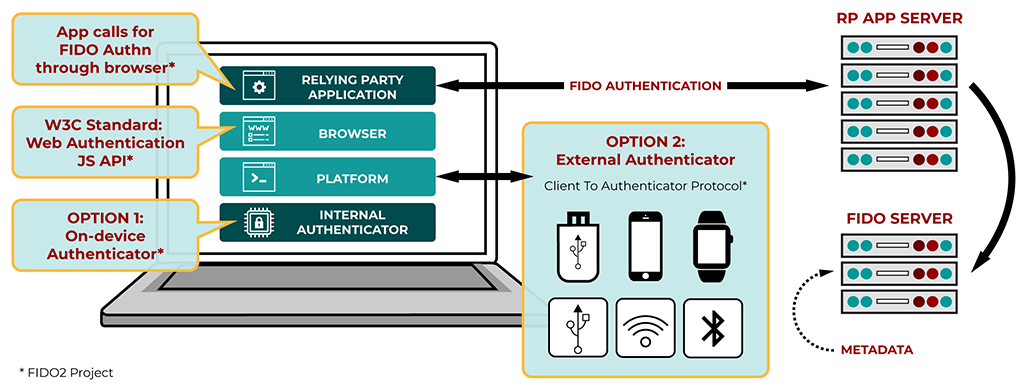
\includegraphics[width=0.9\linewidth]{Figs/FIDO2-Graphic-v2.png}
\caption{\footnotesize \textcopyright FIDO Alliance, from \url{https://fidoalliance.org/specifications/}}
\end{center}
\end{figure}
\end{frame}

\begin{frame}
\small 
\begin{itemize}
 \item \textbf{WebAuthn}: WebAPIと、(端末付属or外部の)認証器・WebApp・サーバ間のハイレイヤのデータフローを規定。
 \item \textbf{CTAP}: ブラウザ・ネイティブAppと外部デバイスの認証器間のローレイヤのプロトコルとAPIを規定。
\end{itemize}
\begin{center}
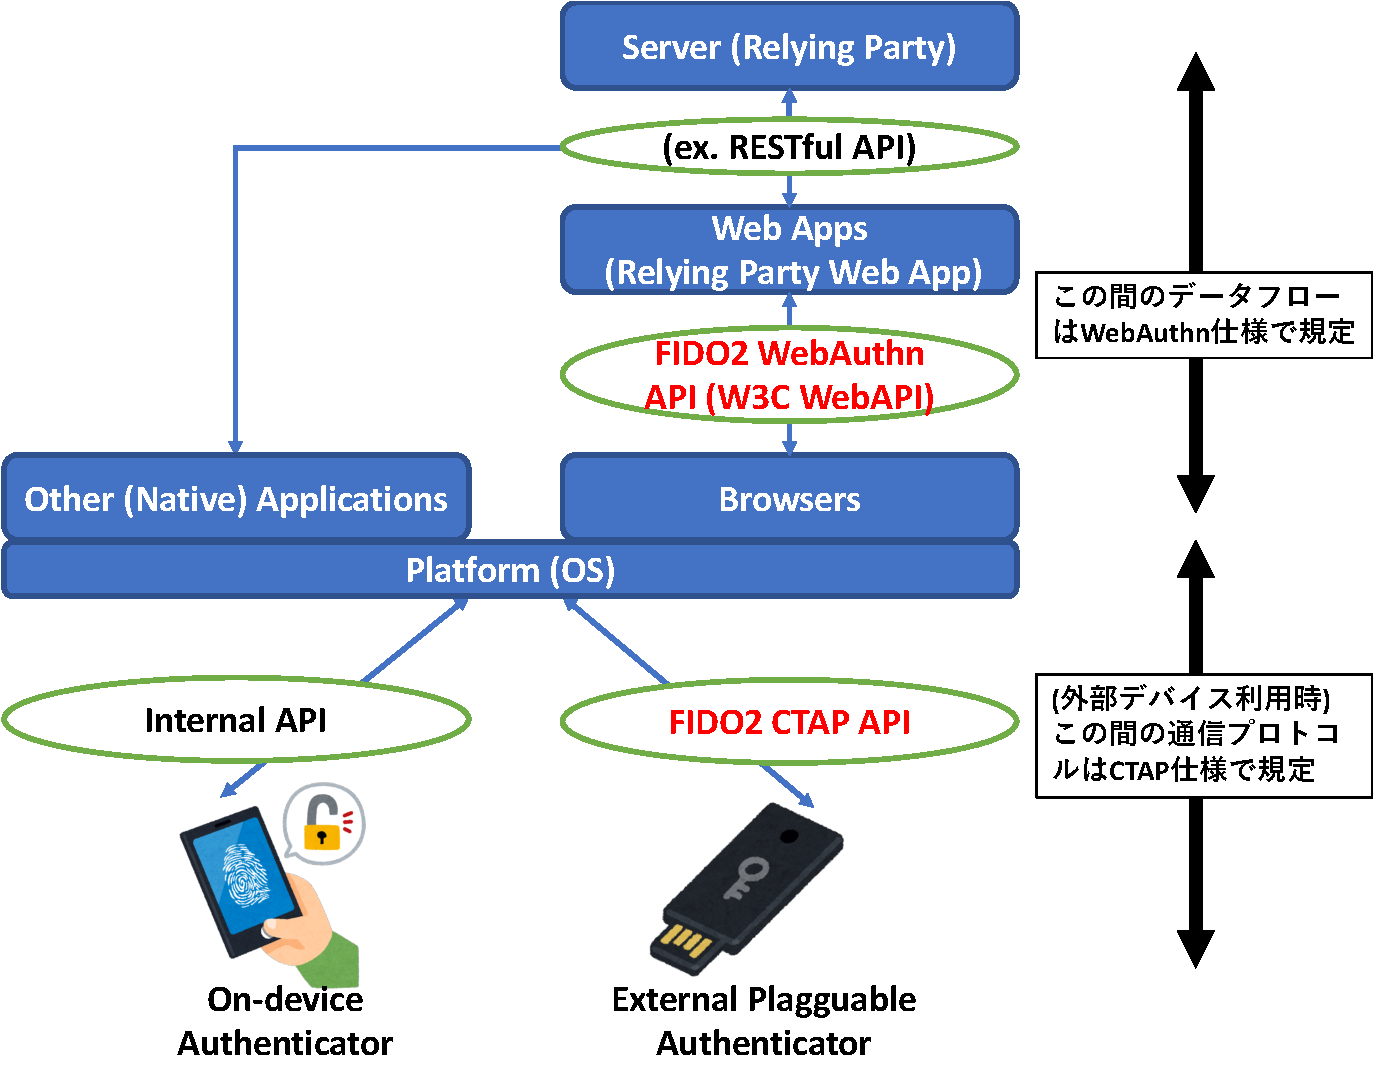
\includegraphics[width=0.8\linewidth]{Figs/FIDO2-spec-structure.pdf}
\end{center}
\end{frame}

\begin{frame}
\begin{block}{FIDO2 WebAuthn}
\end{block}
\end{frame}

\begin{frame}
\begin{block}{FIDO2 CTAP}
\end{block}
\end{frame}

\begin{frame}
\begin{exampleblock}{\small 補足: FIDO1}
\small
FIDO1 (v1.x) は、以下の2つの要素で構成されている。
\begin{itemize}
 \item UAF (Universal Authentication Framework): 生体認証機能を持つFIDO対応端末 (スマートフォン等) で\structure{パスワードレス認証}を行う機構。USB接続などの外部HWセキュリティキーは利用できない。
 \item U2F (Universal 2nd Factor)\footnote[frame]{\scriptsize U2FはFIDO2規格ではCTAP1と改称。FIDO2で追加された仕様はCTAP2と呼ばれる。}: ID・パスワード認証に加えた\structure{2要素認証}を行うのに、外部HWセキュリティキーを利用可能とする機構。
\end{itemize}
FIDO2は、UAFとU2Fを統合し、さらに外部HWキーを用いてもパスワードレス認証可能な、より利便性の高い規格と見做せる。
\end{exampleblock}
 
\end{frame}


\begin{frame}
\frametitle{FIDO2対応デバイス}
\textbf{Security Key by Yubico}
\begin{center}
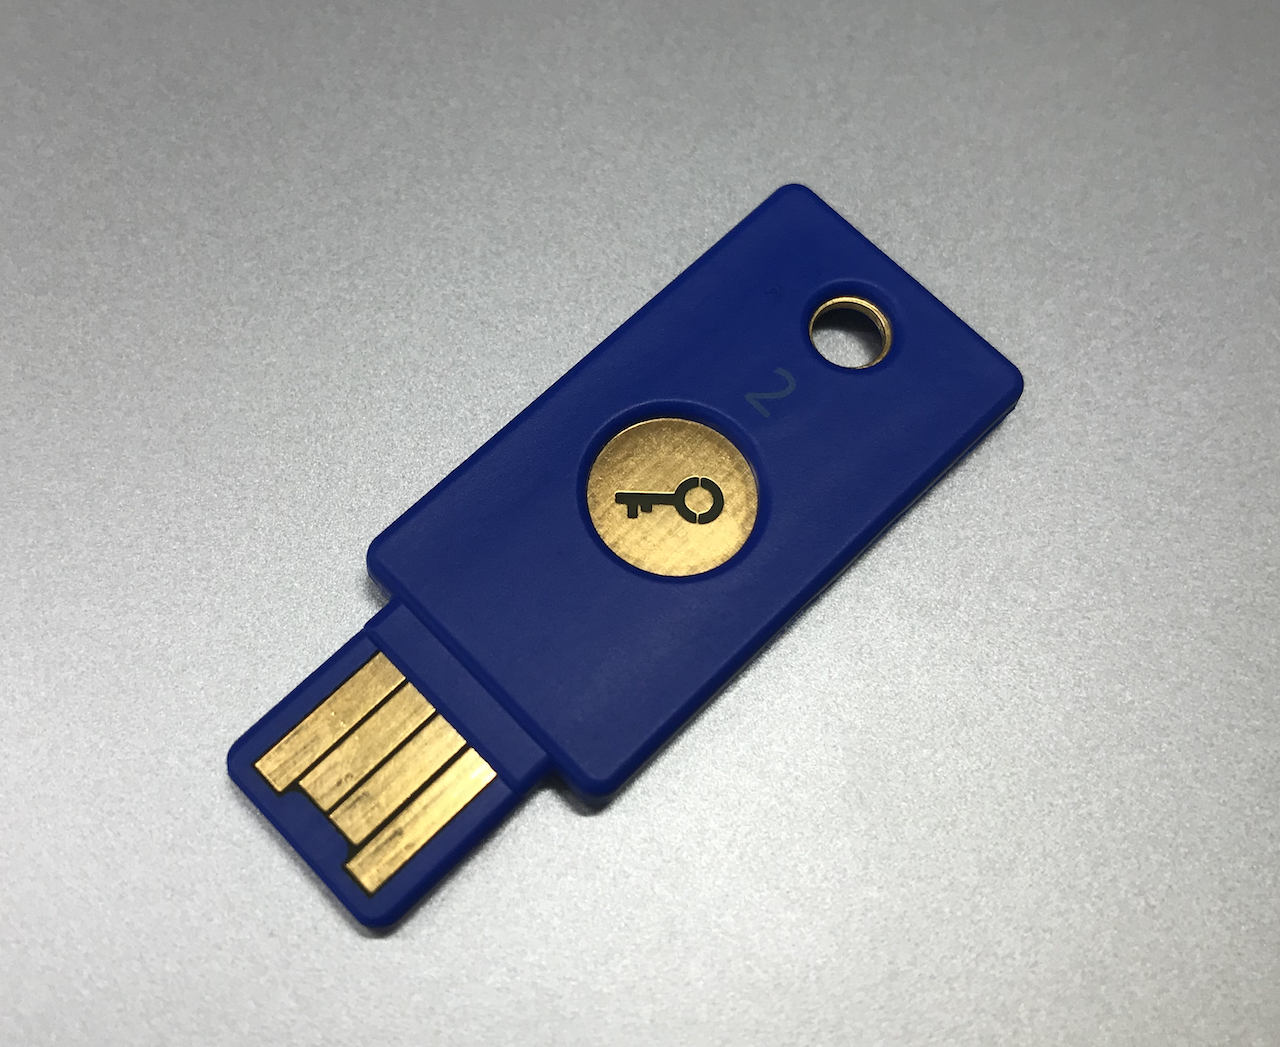
\includegraphics[width=0.6\linewidth]{Figs/security-key-by-yubico.png}
\end{center}
FIDO2専用\footnote[frame]{\scriptsize FIDO2 CTAP1=FIDO1 U2Fには対応}のデバイス
\end{frame}


\begin{frame}{FIDO2標準化状況}

FIDOは業界団体の策定した規格ではあるが、

\begin{itemize}
 \item FIDO2 CTAP: ITU-Tで勧告として国際標準化\footnote[frame]{\scriptsize \url{https://fidoalliance.org/fido-alliance-specifications-now-adopted-as-itu-international-standards/}}
 \item \alert{FIDO2 WebAuthn}: W3Cで勧告として国際標準化\footnote[frame]{\scriptsize \url{https://www.w3.org/2019/03/pressrelease-webauthn-rec.html.ja}}
\end{itemize}

と、認証器とブラウザ間の通信プロトコル、ハイレイヤの認証プロトコルの両者共に国際標準として策定済。

\end{frame}

\begin{frame}
この後、FIDO2 WebAuthnの内容に実際に触れ、最新の認証技術について理解を深めてみよう。\footnote[frame]{\scriptsize 今回はWeb技術から学ぶセキュリティに注力するため、ローレイヤのFIDO2 CTAPについては別の機会で。}
\end{frame}

\section{FIDO2 WebAuthnの構造}
\begin{frame}
\centering
{\Large FIDO2 WebAuthnの構造}
\end{frame}

\begin{frame}

\end{frame}

\section{FIDO2 WebAuthnの中身を解析}
\begin{frame}
\centering
{\Large FIDO2 WebAuthnの中身を解析}
\end{frame}

\begin{frame}
 
\end{frame}

\section{まとめ}
\begin{frame}
\centering
{\huge まとめ}
\end{frame}

\begin{frame}
 
\end{frame}



% %%%%%%%%%%%%%%%%%%%%%%%%%%%%%%%%%%%%%%%%%%%%%%%%%%%%%%%%%%%%%%%%%%%%%%%%%%%%%%%%%%%%%%%%%%%%%%%%%%%
% \backupbegin

% \section{Backup}

% \begin{frame}
 
% \end{frame}

% \begin{frame}
% \frametitle{Appendix}
% This page is not counted.
% \end{frame}
% \backupend
\end{document}
%%%%%%%%%%%%%%%%%%%%%%%%%%%%%%%%%%%%%%%%%%%%%%%%%%%%%%%%%%%%%%%%%%%%%%%%%%%%%%%%%%%%%%%%%%%%%%%%%%%
%%%%%%%%%%%%%%%%%%%%%%%%%%%%%%%%%%%%%%%%%%%%%%%%%%%%%%%%%%%%%%%%%%%%%%%%%%%%%%%%%%%%%%%%%%%%%%%%%%%
%%%%%%%%%%%%%%%%%%%%%%%%%%%%%%%%%%%%%%%%%%%%%%%%%%%%%%%%%%%%%%%%%%%%%%%%%%%%%%%%%%%%%%%%%%%%%%%%%%%
%%%%%%%%%%%%%%%%%%%%%%%%%%%%%%%%%%%%%%%%%%%%%%%%%%%%%%%%%%%%%%%%%%%%%%%%%%%%%%%%%%%%%%%%%%%%%%%%%%%
%%%%%%%%%%%%%%%%%%%%%%%%%%%%%%%%%%%%%%%%%%%%%%%%%%%%%%%%%%%%%%%%%%%%%%%%%%%%%%%%%%%%%%%%%%%%%%%%%%%
%%%%%%%%%%%%%%%%%%%%%%%%%%%%%%%%%%%%%%%%%%%%%%%%%%%%%%%%%%%%%%%%%%%%%%%%%%%%%%%%%%%%%%%%%%%%%%%%%%%
